\documentclass[10pt,a4paper,twocolumn]{article}

\usepackage[utf8]{inputenc}
\usepackage[T1]{fontenc}
\usepackage[margin=1.6cm]{geometry}
\usepackage{graphicx}
\usepackage{xcolor}
\usepackage[colorlinks=true,linkcolor=blue!55!black,urlcolor=blue!55!black,citecolor=blue!55!black]{hyperref}
\usepackage{titlesec}
\usepackage{enumitem}
\usepackage{tabularx}
\usepackage{booktabs}
\usepackage{caption}
\usepackage{microtype}
\usepackage{lmodern}

\titleformat{\section}{\normalfont\bfseries\large\color{blue!45!black}}{\thesection.}{0.5em}{}
\titlespacing*{\section}{0pt}{1.4ex}{0.7ex}

\captionsetup{font=small,labelfont=bf}
\setlength{\columnsep}{0.55cm}
\setlength{\parskip}{0.35em}
\setlength{\parindent}{0pt}

\title{\vspace{-1.6cm}\textbf{HealthWithSevgi}\\[2pt]\Large A Browser-Based ML Education Tool for Healthcare Professionals\\[4pt]\normalsize\textit{Final Project Report --- 2-Page Summary}}
\author{\textbf{EudaLabs Team}\\[6pt]
\normalsize
\begin{tabular}{c@{\hspace{1.4em}}c@{\hspace{1.4em}}c@{\hspace{1.4em}}c@{\hspace{1.4em}}c}
Efe \c{C}elik & Burak Aydo\u{g}mu\c{s} & Batuhan Bayaz\i t & Berat Mert G\"okkaya & Berfin Duru Alkan \\[1pt]
{\footnotesize 202128016} & {\footnotesize 202128028} & {\footnotesize 202228008} & {\footnotesize 202228019} & {\footnotesize 202228005} \\[1pt]
{\footnotesize\textit{PO + Dev}} & {\footnotesize\textit{UX}} & {\footnotesize\textit{Lead Dev + SM}} & {\footnotesize\textit{Dev}} & {\footnotesize\textit{QA Lead}} \\
\end{tabular}\\[6pt]
\normalsize SENG~430 --- Software Quality Assurance\\
\c{C}ankaya University \ $\cdot$ \ Spring 2025--2026}
\date{5 May 2026}

\begin{document}
\maketitle
\thispagestyle{empty}

\noindent\textit{HealthWithSevgi guides healthcare professionals through a seven-step machine-learning pipeline --- from clinical context to ethics audit --- across 20 medical specialties, with no programming required. It ships as a single-container HuggingFace Space pre-built and pulled from the GitHub Container Registry.}

\section{Architecture}
The system is a two-tier web application packaged as a single deployable container. The browser receives a React~18 + Vite + TypeScript single-page application; all stateful operations are delegated to a FastAPI backend over HTTPS. Backend services are singletons attached to \texttt{app.state} and consumed in routers via \texttt{request.app.state.<service>}, organised into three thin route files (\texttt{data\_router}, \texttt{ml\_router}, \texttt{explain\_router}). All session data --- uploaded CSVs, trained models, SHAP values --- lives in a per-process LRU cache; nothing touches a database. The ML engine wraps \texttt{scikit-learn~1.4+}, \texttt{SHAP~0.45+}, and \texttt{XGBoost~/~LightGBM} across eight classifier families. Clinical insights at Step~7 are produced by Google's \textbf{Gemini~2.5~Flash} via the AI~Studio REST API (with an optional MedGemma fall-through on Vertex~AI when configured), and a deterministic template as final fallback when the LLM is unavailable. In production, \texttt{hf-space/main\_hf.py} serves both the API and the static Vite build from a single uvicorn process on port~7860; locally, a Vite proxy forwards \texttt{/api} to a separate uvicorn process. Distribution is via GHCR (\texttt{ghcr.io/eudalabs/\\healthwithsevgi:latest}) with a \texttt{docker-compose.yml} that pulls the pre-built image and falls back to a local multi-stage build.

\begin{figure*}[t]
  \centering
  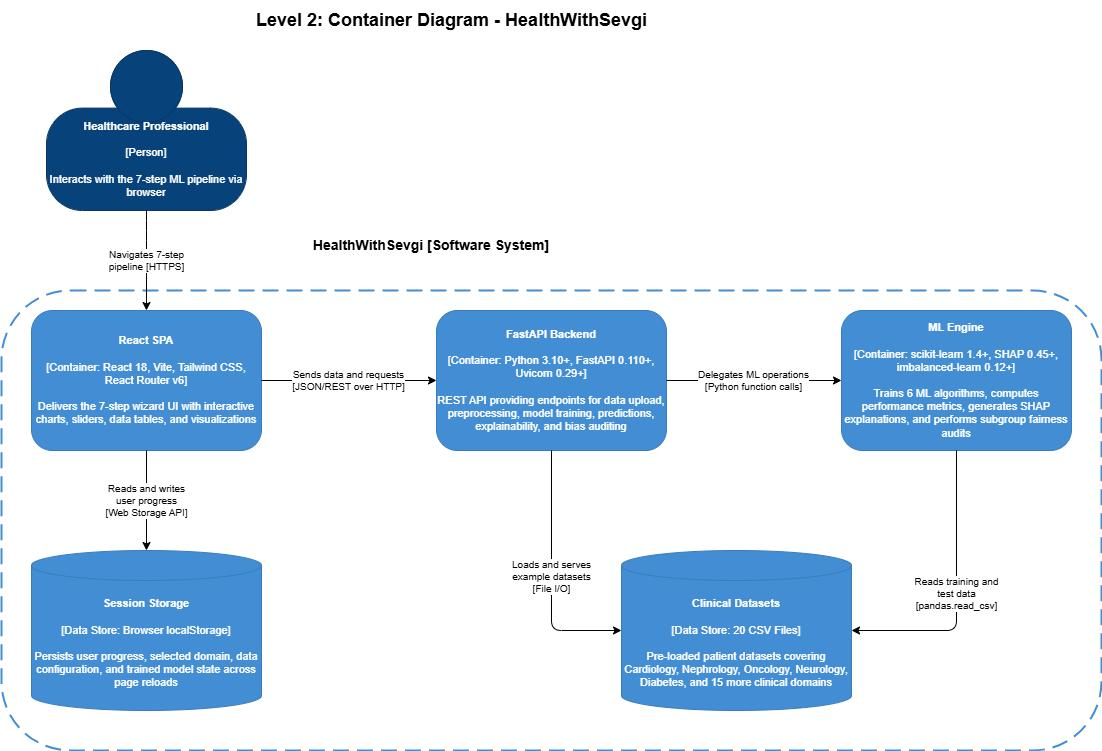
\includegraphics[width=0.92\linewidth]{../diagrams/c4-level2-container.drawio.pdf}
  \caption{C4 Level-2 Container view of HealthWithSevgi. Source under \texttt{docs/drawio/}.}
  \label{fig:c4-level2}
\end{figure*}

\section{Key Decisions}
\begin{itemize}[leftmargin=*,itemsep=0.25ex,topsep=0pt]
  \item \textbf{No database.} All clinical data stays in-memory and is evicted as the LRU fills. Eliminates a class of privacy risks and removes a dependency for graders running clean-room.
  \item \textbf{Single-container deployment.} The same image runs locally via \texttt{docker compose up}, on HuggingFace Spaces, and on a clean grader machine. \texttt{main\_hf.py} mounts the Vite build under uvicorn so there is no second process to supervise.
  \item \textbf{Gemini~2.5~Flash with thinking-aware parsing.} A brief migration to Gemma~4 (v1.5.8) was reverted in favour of Gemini~2.5~Flash for stability. The response parser still drops parts marked \texttt{thought=true} so any chain-of-thought tokens never leak into the clinical assessment card.
  \item \textbf{Lazy-loaded wizard steps.} Steps~2 through~7 are dynamic-imported via \texttt{React.lazy}. Recharts is no longer eagerly preloaded at landing --- landing JS dropped by 70~KiB and Lighthouse SEO climbed from 91 to 100.
  \item \textbf{Accessibility without opacity.} Locked wizard steps formerly used \texttt{opacity: 0.45} to indicate disabled state; opacity stacked with the parent surface and broke the WCAG~1.4.3 contrast target. Replaced with \texttt{var(--text-secondary)} which clears AA at 5.85:1.
  \item \textbf{GHCR-first compose.} \texttt{docker-compose.yml} reaches for the pre-built image first; the local build context is a fallback. Graders need only \texttt{docker compose up} --- no source checkout.
\end{itemize}

\section{Challenges}
\textbf{Step-7 LLM reliability.} The original 45~s axios + 45~s server timeout was too tight for the Step-7 reasoning calls: long ethics prompts occasionally crossed 60~s and the frontend rendered empty cards on every other request. Resolution: backend HTTP timeout raised to 200~s, one jittered retry on \texttt{ReadTimeout~/~429~/~5xx}, axios bumped to 450~s, and a graceful \emph{``assessment unavailable, reload to retry''} alert when the template fallback fires instead of a blank card. Verified across five consecutive multi-task calls (15~/~15 successful Gemini responses).

\textbf{Sprint-4 retrospective debt.} Five bugs surfaced in the Sprint-4 retro (\texttt{SCRUM-217..221}, 11~pts) --- a missing \texttt{ErrorBoundary} around lazy steps, silent error suppression in Step~6, a parallel-coordinates crash on null metric, and two related null-handling regressions. They were re-prioritised into Sprint~5 and \emph{shipped in the first half} of the sprint window so polish and user-testing landed on a stable trunk.

\textbf{Cross-browser regression caught late.} UT-03 caught a Safari-specific viewport regression in the parallel-coordinates chart only at audit time. The fix was a one-line \texttt{min-height}; the discovery cost a half-day. The standing recommendation is a Playwright matrix in CI running Chrome~/~Firefox~/~Safari~/~Edge on every PR.

\textbf{20 specialties $\times$ 7 steps $\times$ 3 CSV variants.} Building enough end-to-end coverage for a five-person team to credibly claim \emph{``no crashes across all clinical specialties''} required automation: 140 cases for full-domain coverage and 21 cases for the 3-CSV regression suite. Together they document 161~/~161 passing cases with zero failures (\texttt{Sprint5\_Full\_Domain\_Coverage.pdf}, \texttt{Sprint5\_E2E\_Regression.pdf}).

\section{Lessons Learned}
\begin{itemize}[leftmargin=*,itemsep=0.25ex,topsep=0pt]
  \item \textbf{Book user-testing windows at the \emph{start} of the sprint, not the end.} Recording and signed consent slipped to the final 48~hours because both were scheduled after polish. The fix is administrative: lock the participant slot during sprint planning.
  \item \textbf{One non-CS user is the floor, not the bar.} P1 returned 7~/~7 task pass with SUS~90, but a single observation cannot triangulate a population. Two follow-up sessions (clinician + administrator) are queued for any post-academic continuation.
  \item \textbf{Quality scores need a CI floor.} Lighthouse Perf~91~/~A11y~100~/~BP~100~/~SEO~100 was achieved manually. Without a GitHub Action gating \texttt{main} on a Lighthouse threshold, any future contributor can silently regress jury-grade scores. The proposed gate is Perf~$\geq$~85 and A11y~$\geq$~95, evaluated against the production HF build.
  \item \textbf{Documentation is a deliverable, not a chore.} Frontend JSDoc and backend \texttt{interrogate} both reached 100~\% in Sprint~5. Instituting the rule from Sprint~1 would have spread the cost across five sprints rather than concentrating it in the last one.
  \item \textbf{Reasoning models need different timeouts than chat models.} The Step-7 incident is the durable lesson: any LLM with chain-of-thought reasoning needs an SLA per call that accounts for the reasoning pass, plus parser-level filtering of \texttt{thought} parts before they reach the user.
\end{itemize}

\vspace{0.6ex}
\hrule height 0.4pt
\vspace{0.4ex}
{\footnotesize\textit{Live demo:} \url{https://0xbatuhan4-healthwithsevgi.hf.space/} \quad
\textit{Source:} \url{https://github.com/EudaLabs/HealthWithSevgi} \quad
\textit{Wiki:} \url{https://github.com/EudaLabs/HealthWithSevgi/wiki} \quad
\textit{Container:} \url{https://github.com/EudaLabs/HealthWithSevgi/pkgs/container/healthwithsevgi}}

\end{document}
